\section{Basics of event-driven ABS}
In this section we derive step-by-step the basics of event-driven ABS using the SIR model, as introduced in Chapter \ref{sec:sir_model}, with an event-driven approach. This is in stark contrast to the time-driven implementation in Chapter \ref{sec:timedriven_firststep}. The solutions are quantitatively equal as they produce the same class of dynamics. Qualitatively they fundamentally differ though in terms of expressivity and performance as we will see in the discussion.

The basics of event-driven ABS are the concept of agent identity, events and event-scheduling. We introduce them step-by-step using various Monads and then generalise to a \textit{tagless final} approach, which has various benefits as pointed out in the respective section. 

\subsection{An event-driven SIR}
Before we can derive implementation concepts, we first need to discuss how an event-driven SIR model works, as inspired by \cite{macal_agent-based_2010}. Fundamentally, what is required is to transform all time-dependent behaviour and agent interactions into the reception and scheduling of events. For the SIR this should be trivial and straight-forward, taking inspiration from the time-driven implementation, where we simply translate the occurrences of events generated by \textit{occasionally} into scheduled events. For agent interactions we also use events, making this more explicit than in the time-driven approach. As already pointed out, assuming that events have a receiver and a scheduling time given as $\Delta t$ relative to the current simulation time, we end up with three event-types:

\begin{enumerate}
	\item \textbf{MakeContact} - is used to let susceptible agents pro-actively make contact with $\beta$ (contact rate) other agents per 1 time-unit.
	\item \textbf{Contact$_{Sender, \ SIRState}$} - is used to make contact between agents where agents reveal their state by sending or replying with their current state.
	\item \textbf{Recover} - is used to let infected agents pro-actively recover after the given $\delta$ (illness duration). 
\end{enumerate}

Now we can give a concise definition of all three agent behaviours:

\paragraph{Susceptible Agent}
\begin{itemize}
	\item A susceptible agent initially schedules a \textit{MakeContact} event with $\Delta t = 1$ to itself.
	\item When receiving \textit{MakeContact}, the agent sends a \textit{Contact} event to $\beta$ (contact rate) random other agents with $\Delta t = 0$ and \textit{SIRState} of \textit{Susceptible}, resulting in these events to be scheduled immediately. Further, the agent schedules \textit{MakeContact} with $\Delta t = 1$ to itself, to keep the pro-active process of making contact with other agents active.
	\item When the agent receives a \textit{Contact} event, it checks if it is from an infected agent (\textit{SIRState} is \textit{Infected}). If the event is not from an infected agent, it ignores it, otherwise it becomes infected with a given probability.
\end{itemize}

\paragraph{Infected Agent}
\begin{itemize}
	\item An infected agent initially schedules a \textit{Recover} event to itself, with an exponentially distributed random $\Delta t$ of $\delta$ (illness duration).
	\item When the agent receives a \textit{Contact} event, it checks if it is from a susceptible agent (\textit{SIRState} is \textit{Susceptible}). If the event is not from a susceptible agent, it ignores it, otherwise it simply replies to this susceptible agent with a \textit{Contact} event with $\Delta t = 0$ and and \textit{SIRState} of \textit{Infected}.
\end{itemize}

\paragraph{Recovered Agent}
The recovered agent does not change any more, reacts to no incoming events and schedules no events - it stays constantly \textit{Recovered} forever.

\medskip

It is easy to see that this behaviour emulates the time-driven one and is qualitatively equivalent and indeed in Figure \ref{fig:sir_eventdriven_dynamics} it is also visually clear that it produces similar dynamics. A striking difference are the small spikes and steps in the dynamics, which stem from the fact that time advances discretely and not continuous as in the time-driven implementation. In Chapter \ref{ch:sir_invariants}, we use property-based testing to show that the different implementations indeed produce similar distributions in their dynamics, thus putting the claim that both implementations are qualitatively equal on a much more robust ground.

\begin{figure}
	\centering
	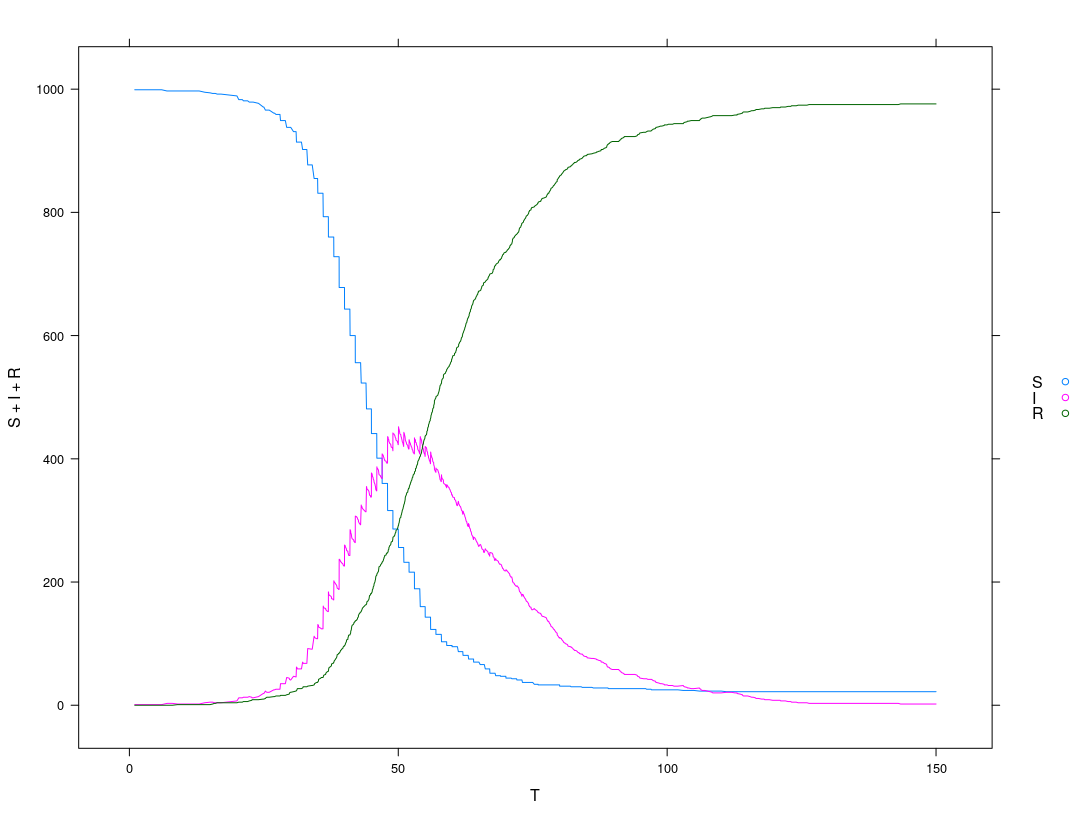
\includegraphics[width=0.7\textwidth, angle=0]{./fig/eventdriven/sir_eventdriven.png}
	\caption{Dynamics of the event-driven SIR model. Population Size $N$ = 1,000, contact rate $\beta = \frac{1}{5}$, infection probability $\gamma = 0.05$, illness duration $\delta = 15$ with initially 1 infected agent. Simulation run for 150 time-steps.}
	\label{fig:sir_eventdriven_dynamics}
\end{figure}

\subsection{First steps}
We can now start to discuss the concepts from an implementation perspective. First, we need to make the concept of an event explicit: they are of a given type, have a receiver and a time-stamp in \textit{absolute} simulation time when they shall be scheduled. We keep the event-type polymorphic and represent the receiver by an \textit{AgentId} which is a simple \textit{Int}. For efficient scheduling, the events are kept in a priority-queue \footnote{We are using the \textit{Data.PQueue.Min} implementation from the \textit{pqueue} package.}, sorted ascending by the time-stamp. Thus we define the following:

\begin{HaskellCode}
type Time        = Double
type AgentId     = Int
data QueueItem e = QueueItem e AgentId Time

-- the event priority-queue
type EventQueue e = PQ.MinQueue (QueueItem e)

-- implement Ord for QueueItem for acended sorting
instance Ord (QueueItem e) where
  compare (QueueItem _ _ t1) (QueueItem _ _ t2) = compare t1 t2
\end{HaskellCode}

Next, we define a polymorphic type for our agent. As already pointed out, we will switch to the direct use of \textit{MSF} instead of BearRivers \textit{SF}. As input, the polymorphic event-type \textit{e} is used, because in event-driven ABS agents receive events, which drive the simulation. As output, the polymorphic output-type \textit{o} is used, which will be instantiated to a specific monomorphic type in the SIR model below. The question is now, what Monad shall be used. For scheduling purposes (and maybe also some models require it in general), agents should be able to \textit{read} the current simulation time: this is accomplished through a \textit{ReaderT Time}. Further, agents should be able to \textit{read} the identities of the other agents available in the simulation so they can schedule events to them when necessary: this is accomplished through a \textit{ReaderT [AgentId]}. Most importantly, agents have to be able to schedule events, meaning they have to be able to \textit{write} the events into some sink where they are accumulated for scheduling: this is accomplished through a \textit{WriterT [QueueItem e]}. Finally, the transformer stack needs to be extendible by other Monads, specified in concrete models like the SIR below, so we add another polymorphic type \textit{m}, indicating the closing Monad (stack).

\begin{HaskellCode}
type ABSMonad m e   = ReaderT Time (WriterT [QueueItem e] (ReaderT [AgentId] m))
type AgentMSF m e o = MSF (ABSMonad m e) e o
\end{HaskellCode}

Note that BearRivers \textit{SF} has also a \textit{ReaderT Double} as the innermost Monad but we deliberately avoided its use because the intended semantics of an \textit{SF} are different: the value in the \textit{ReaderT} of the \textit{SF} represents the sampling time-delta and not the absolute time, as in the event-driven case.

We can already implement a few polymorphic functions, operating on the given Monad stack. First, we implement a function \textit{allAgentIds} which simply returns the \textit{AgentId} of all agents, the contents of the \textit{ReaderT [AgentId]}. Second, we implement a function \textit{scheduleEvent} which allows to schedule a given event to a given receiver into the future given a specific time-delay, relative to the current simulation time.
 
\begin{HaskellCode}
allAgentIds :: Monad m => (ABSMonad m e) [AgentId]
allAgentIds = lift (lift ask)

scheduleEvent :: Monad m
              => e                 -- ^ event
              -> AgentId           -- ^ receiver
              -> Double            -- ^ time-delay
              -> (ABSMonad m e) ()
scheduleEvent e aid dt = do
  -- get current simulation time
  t <- ask
  -- construct queue item
  let q = QueueItem e aid (t + dt)
  -- write/append (tell) to the WriterT (QueueItem e)
  lift (tell [q])
\end{HaskellCode}

Processing events can also be implemented generically and is straight forward, thus we only discuss the subtleties. For efficient lookup of event receivers all agents are organised into an \textit{IntMap}, which also holds the current output of the agent, to allow sampling of the domain-state. In general, the domain-state is highly model specific, thus a generic implementation needs to offer some mechanism to update the domain-state after an event, a process we named domain-state sampling. Our approach is to call a function which receives the agent map and returns a new domain-state for the current event/time-step. These domain-states are appended to an infinite list which forms the output of the simulation.

The events are then processed in the order provided by the queue and each event is executed with the given receiver. Running a receiver is simply achieved using the agent map, where a reviver is looked up and its \textit{MSF} is evaluated with the given event as input and the resulting monadic actions executed with the given information.
 
\subsection{Parametrising for SIR}

\begin{HaskellCode}
data SIRState
  = Susceptible
  | Infected
  | Recovered
  
data SIREvent 
  = MakeContact
  | Contact AgentId SIRState
  | Recover 
\end{HaskellCode}

\begin{HaskellCode}
type SIRMonad g = ABSMonad (Rand g) SIREvent
type SIRAgent g = AgentId -> (SIRMonad g) (AgentMSF (SIRMonad g) SIREvent SIRState)

sirAgent :: RandomGen g 
         => Int         -- ^ the contact rate
         -> Double      -- ^ the infectivity
         -> Double      -- ^ the illness duration
         -> SIRState    -- ^ the initial state of the agent
         -> SIRAgent g
sirAgent beta gamma delta Susceptible aid = do
  -- on start
  scheduleMakeContact aid 1
  return (susceptibleAgent aid beta gamma delta)
sirAgent _ _ delta Infected aid = do
  -- on start
  scheduleRecovery aid delta
  return (infectedAgent aid)
sirAgent _ _ _ Recovered _ = 
  return recoveredAgent

scheduleMakeContact :: RandomGen g => AgentId -> Double -> (SIRMonadT g) ()
scheduleMakeContact aid = scheduleEvent MakeContact aid

scheduleRecovery :: RandomGen g => AgentId -> Double -> (SIRMonadT g) ()
scheduleRecovery aid ild = do
  dt <- (lift . lift . lift) (randomExpM (1 / ild))
  scheduleEvent Recover aid dt
\end{HaskellCode}

Next, we show the full implementation of the susceptible agent behaviour. The infected and recovered behaviours are conceptually equivalent and thus not shown here.

\begin{HaskellCode}
susceptibleAgent :: RandomGen g 
                 => AgentId
                 -> Int
                 -> Double
                 -> Double
                 -> SIRAgentMSF g
susceptibleAgent aid cor inf ild = 
    switch
      susceptibleAgentInfected
      (const (infectedAgent aid))
  where
    susceptibleAgentInfected :: RandomGen g 
                             => MSF
                                (SIRMonadT g) 
                                SIREvent
                                (SIRState, Maybe ()) 
    susceptibleAgentInfected = proc e -> do
      ret <- arrM handleEvent -< e
      case ret of
        Nothing -> returnA -< (Susceptible, ret)
        _       -> returnA -< (Infected, ret)

    handleEvent :: RandomGen g => SIREvent -> (SIRMonadT g) (Maybe ())
    handleEvent (Contact _ Infected) = do
      r <- (lift . lift . lift) (randomBoolM inf)
      if r 
        then do
          scheduleRecovery aid ild
          return (Just ())
        else return Nothing

    handleEvent MakeContact = do
      ais       <- allAgentIds
      receivers <- (lift . lift . lift) (forM [1..cor] (const (randomElem ais)))
      mapM_ makeContactWith receivers
      scheduleMakeContact aid makeContactInterval
      return Nothing

    handleEvent _ = return Nothing

    makeContactWith :: AgentId -> (SIRMonadT g) ()
    makeContactWith receiver = 
      scheduleEvent (Contact aid Susceptible) receiver 0
\end{HaskellCode}

\subsection{Tagless Final}
The main benefit of a \textit{tagless final} approach is that it is a solution to the expression problem \cite{kiselyov_typed_2012}: it is possible to add new interpreters of an embedded language and add new functionality without breaking the existing implementations. Interpretation in our case means that we can use different underlying Monads to run the agents in: if we want to guarantee purity, no IO Monad shall be used in  the interpreter. Otherwise when concurrency with a lock-based approach or a lock-free approach is required IO or STM can be used in the underlying interpreter. Also, for reproducible unit testing testing, one can write custom test-interpreters where methods always return a-priori known results, similar to mocking.
Adding new functionality is less an issue here but might become highly important when designing a more general ABS library in Haskell, building on the \textit{tagless final} approach. It would allow the user of such a library to extend existing agents or default behaviour with new, custom-built methods, without breaking the existing ones.